\subsection{Hipótese 1}
\label{sec:resultados-hipotese-1}

Primeiramente vamos avaliar a hipótese 1.
A estratégia é simples: para cada um dos cursos (DA e DS), vamos segmentar o conjunto de dados em dois sub-conjuntos, um das aulas referentes a ferramentas; o outro com o complemento.
Em seguida, aplicamos um teste de hipótese estatístico para avaliar a hipótese nula de que a média $\mu_f$ da população de todas as aulas referentes a ferramentas é igual à média $\mu_{\neg f}$ da população de todas as demais aulas.
Ou seja,
\begin{align*}
	H_0&: \mu_f = \mu_{\neg f} \\
	H_a&: \mu_f > \mu_{\neg f}
\end{align*}

O conjunto de dados pré-processado já contém a informação de que um dado componente refere-se a uma ferramenta ou não (coluna \foreign{tool} na Figura~\ref{fig:dataset}).
Assim, podemos segregar o conjunto de dados segundo esse critério.

\begin{figure}[b]
	\centering
	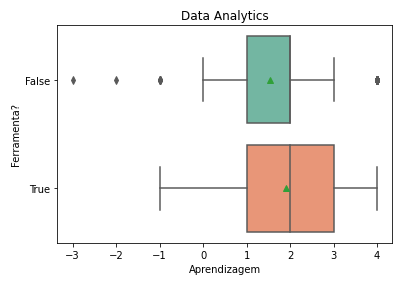
\includegraphics[width=0.45\textwidth]{da-boxplot-by-tool}\hfill
	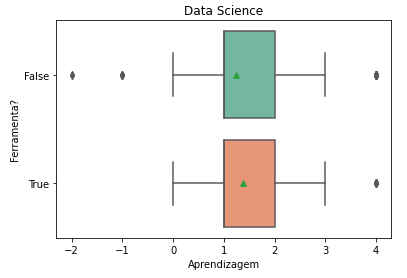
\includegraphics[width=0.45\textwidth]{ds-boxplot-by-tool}
	\caption{Distribuição da aprendizagem nos cursos de DA (esquerda) e DS (direita) para as aulas de ferramentas (\foreign{true} no eixo vertical) e as demais. Os triângulos verdes indicam a média amostral.}
	\label{fig:dist-hipotese-1}
\end{figure}

Note que a hipótese 1 baseia-se na suposição de que podemos calcular a média das aprendizagens.
Há décadas discute-se sobre a possibildiade de interpretar a escala Likert como variável numérica.
Considerando que os valores de $q_\text{antes}$ (idem para $q_\text{depois}$) guardam entre si uma relação de ordenação, a partir da qual é possível construir um espaço métrico \cite[cap.~27]{Barata2020}, mais as recomendações de \cite{Harpe2015}, consideramos válido assumir que $a$ (equação~\ref{eq:a}) é de fato numérica e que, por isso, $\bar a$, $\mu_f$ e $\mu_{\neg f}$ existem.

A Figura~\ref{fig:dist-hipotese-1} representa a distribuição dos valores de aprendizagem $a$ para os sub-conjuntos: \foreign{true} refere-se às aulas de ferramenta.

A Tabela~\ref{tab:dist-hipotese-1} apresenta as médias, desvio-padrão e erro-padrão da média (nível de significância de 5\%) para cada um dos sub-conjuntos dos cursos de DA e DS.
Vemos, por exemplo, que para DA a média amostral de aprendizagem nas aulas de ferramentas é de $1,9\pm{0,1}$, ou seja, ela reside no intervalo [1,8;2,0] com confiança de 95\%, que não contém a média da aprendizagem nas demais aulas.
Observação análoga pode ser feita para DS, à direita na tabela.
Esse resultado é um indício de que realmente há uma diferença entre as médias populacionais, mas para fazermos essa afirmação precisamos do teste t.

\begin{table}
	\caption{Tamanho da amostra (\#), média (e erro padrão) e desvio-padrão de cada sub-conjunto de DA (esquera) e DS (direita).}
	\label{tab:dist-hipotese-1}
	\centering
	\begin{minipage}{0.45\textwidth}
		\begin{tabular}{lrrr}
			\toprule
			\multicolumn{4}{c}{Data Analytics}\\
			Ferramenta? & \# & $\bar{a}$ & $s_a$ \\
			\midrule
			Sim &  408 & $1,9\pm 0,1$ & 1,1 \\
			Não & 1470 & $1,55 \pm 0,05$ & 1,1 \\
			\bottomrule
		\end{tabular}
	\end{minipage}\hfill
	\begin{minipage}{0.45\textwidth}
		\begin{tabular}{lrrr}
			\toprule
			\multicolumn{4}{c}{Data Science}\\
			Ferramenta? & \# & $\bar{a}$ & $s_a$ \\
			\midrule
			Sim &  232 & $1,4\pm 0,1$ & 1,0 \\
			Não & 1531 & $1,23\pm 0,04$ & 0,9 \\
			\bottomrule
		\end{tabular}
	\end{minipage}
\end{table}

Antes de efetuarmos o teste da hipótese 1, vamos checar se ambos os sub-conjuntos apresentam distribuição normal.
Para isso utilizamos o teste de Lilliefors com nível de significância de 5\% (valor-padrão na literatura).
O resultado é um valor-$p$ bastante inferior ao nível de significância, o que significa que a distribuição \emph{não} é normal.
Apesar disso, segundo~\cite[p.~259]{Triola2005} é possível realizar o teste t a seguir mesmo que a amostra não provenha de uma distribuição normal, desde que a amostra tenha tamanho maior do que 30, que é o nosso caso: o menor dos sub-conjuntos tem 232 observações.

Executamos o teste t de duas amostras independentes com populações cuja variância é desconhecida.
Para DA obtivemos $\text{valor-}p \approx 4\times10^{-8}$ com a estatística t positiva: veja a Tabela~\ref{tab:hipotese-1}.
Isso significa que a probabilidade de observarmos uma distribuição amostral com a média $\bar a = 1,9\pm 0,1$, sob a suposição de que essa amostra tem origem numa população cuja média $\mu_f = 1,55\pm 0,05$, é da ordem de $4\times10^{-8}$.
Ou seja, é improvável.
Na verdade, é mais improvável do que o que originalmente escolhemos aceitar, o nível de significância de 5\%.
Logo, podemos rejeitar $H_0$ e afirmar que de fato $\mu_{f} > \mu_{\neg f}$.

Em palavras, os alunos aprendem mais nas aulas referentes a ferramentas do que nas demais aulas de DA.


Análise análoga pode ser feita para DS (Tabela~\ref{tab:hipotese-1}): o valor $p$ é inferior ao nível de significância e a estatística t é positiva, significando que também para DS os alunos aprendem mais nas aulas referentes a ferramentas do que nas demais.

À luz da teoria do valor da expectativa, podemos argumentar que as aulas de ferramentas oferecem aos alunos uma relação explícita (instrumentalidade) com as demandas de vagas de postos de trabalho, de modo que a expectativa de obter um emprego (valência) promove no aluno motivação intrínseca para aprender.
Essa relação não é tão evidente nas demais aulas, levando a uma instrumentalidade menor e, por conseguinte, menor motivação para aprender.


\begin{table}
	\centering
	\caption{Resultado do teste da hipótese 1 nos cursos DA e DS.}
	\label{tab:hipotese-1}

	\begin{tabular}{lcc}
	\toprule
	Curso & Valor $p$   & Estatística $t$ \\
	\midrule
	DA    & $<10^{-11}$ & $7,24$ \\
	DS    & $0,03$      & $2,13$ \\ 
	\bottomrule
	\end{tabular}
\end{table}

% britannica.com/topic/motivation/Behavioristic-approaches-to-motivation
Essa aprendizagem aprimorada nas aulas de ferramentas pode ser, ainda, um efeito do chamado condicionamento operante \cite{Petri}, uma abordagem comportamentalista da motivação: a utilização das ferramentas leva a resultados concretos que, por sua vez, motivam aprendizagens subsequentes.

Independentemente do processo cognitivo, intangível à experiência, o fato é que há diferença.
Isso sugere que podemos utilizar essa motivação nas demais aulas.
Duas possibilidades nos ocorre: (1) desenvolver as demais aulas utilizando as ferramentas, se possível (aprendizagem significativa); e (2) tornando evidente, por discurso, a relação com os requisitos do mercado (teoria do valor da expectativa).